%http://mathematica.stackexchange.com/questions/11350/xkcd-style-graphs
\documentclass[12pt]{article}
\usepackage[authoryear]{natbib}
\usepackage[margin=1.0in]{geometry}
\usepackage{pseudocode}
\usepackage{mathtools}
\usepackage{datetime}\usepackage{hyperref}
\usepackage{amsmath}
\usepackage{amsfonts}
\usepackage{graphicx}
\usepackage{bookman}
\usepackage{pgfplotstable}%for generating latex from csv files
\usepackage{booktabs}
\usepackage{cmbright}

%\usepackage{ccfonts,eulervm}
%\usepackage[T1]{fontenc}

% \usepackage{ccfonts}
% \usepackage[T1]{fontenc}

\title{``A Useful Representation For Time Invariant Functions and
A Solution Strategy for Occasionally Binding Constraints in Rational Expectations Models''}
\date{\today -- \currenttime}



\author{Gary S. Anderson}
\newcommand{\xtFuncTI}{\mathcal{X}(x,\epsilon)}
\newcommand{\XtFuncTI}{\mathbf{X}(x)}

\newcommand{\xtFunc}[1]{\mathcal{X}{#1}}
\newcommand{\XtFunc}[1]{\mathbf{X}{#1}}



\newcommand{\discr}[1]{\mathcal{D}^{#1}(x_{t-1},\epsilon_t)}

\newcommand{\XZPair}[1]{(\mathcal{X}^{#1},\mathcal{Z}^{#1})}
\newcommand{\XZPairG}[1]{(\mathcal{X}^{#1}(x^g),\mathcal{Z}^{#1}(x^g))}
\newcommand{\xIter}[2]{\mathcal{X}^{#1}(#2)}
%\newcommand{\zNow}[1]{z^{#1}_0(x_{t-1},\epsilon_t)}
%\newcommand{\ZNow}[3]{\mathcal{Z}^{#1}_{#2}(x_{#3})}
\newcommand{\zNow}[1]{z^{#1}(x_{t-1},\epsilon_t)}
\newcommand{\ZNow}[3]{\mathcal{Z}^{#1}(x_{#3})}

\newcommand{\xNow}[1]{x^{#1}_t(x_{t-1},\epsilon_t)}
\newcommand{\xNowtp}[1]{x^{#1}_{t+1}(x_{t-1},\epsilon_t)}
\newcommand{\XNow}[3]{\mathcal{X}^{#1}_{#2}(x_{#3})}








\newcommand{\sForSum}{{\nu}}
\newcommand{\rcpC}{{\mathbf{c}}}

\newcommand{\xtVec}{  \begin{bmatrix}
    q_t\\r_{t}\\r_{ut}
  \end{bmatrix}
}
\newcommand{\xtPVec}{  \begin{bmatrix}
    q_{t+1}\\r_{t+1}\\r_{ut+1}
  \end{bmatrix}
}
\newcommand{\xtMVec}{  \begin{bmatrix}
    q_{t-1}\\r_{t-1}\\r_{ut-1}
  \end{bmatrix}
}
\newcommand{\expctEps}[1]{\mathcal{E}_{\epsilon} \left [#1 \right ]}
\newcommand{\expct}[2]{E_{#1} \left [#2 \right ]}
\newcommand{\expc}[1]{\mathcal{E} \left [#1 \right ]}
\newcommand{\expcK}[2]{\mathcal{E}^{#1} \left [#2 \right ]}
\newcommand{\xsln}[1]{\mathbb{X} \left [#1 \right ]}
\newcommand{\xslnK}[2]{\hat{\mathbb{X}}^{#1} \left [#2 \right ]}
\newcommand{\xpth}[2]{\mathfrak{X}_{#1} \left [#2 \right ]}
\newcommand\infNorm[1]{\left\lVert#1\right\rVert_\infty}
\newcommand\twoNorm[1]{\left\lVert#1\right\rVert_2}
%\newcommand{\inorm}[1]{\left\lVert#1\right\rVert_\infty}

% \newcommand{\forPhi}{\begin{bmatrix}
% \psi_\epsilon&\psi_z
% \end{bmatrix}}
% \newcommand{\phiMult}{\phi \psi_\epsilon}
% \newcommand{\bMult}{B x_{-1} + \phiMult}
\newcommand{\phiMultBoth}[1]{
	\phi (\psi_\epsilon \epsilon_t +\psi_z z_0^#1(x_{-1},\epsilon_t))}
\newcommand{\bMultBoth}[1]{B x_{-1} + \phiMultBoth{#1}}


\newcommand{\bForOne}{\bMultBoth{1}
}

% \newcommand{\bForTwo}{\bMultBoth{2}+
% F \phi  \psi_z  
% Z_0^1(x_0^2(x_{-1}))   
% }



\newcommand{\compSlack}{z_0^1(x_{-1},\epsilon_t) \left ( \bar{x} -x\right )=0\\ z_0^1(x_{-1},\epsilon_t)> 0}
% \begin{gather*}
% 0= x_t-(B x_{t-1}+ \phi \psi_\epsilon\epsilon_t + \phi \psi_z 
% \xpt{z_{t}(x_{t-1},\epsilon_t)    } )
% \end{gather*}

\newcommand{\xpt}[1]{#1}


\makeatletter
\@ifundefined{newblock}{%
 \def\newblock{\hskip .11em plus .33em minus .07em} % important line
}
\makeatother


\makeatletter
\pgfplotsset{
    /pgfplots/table/omit header/.style={%
        /pgfplots/table/typeset cell/.append code={%
            \ifnum\c@pgfplotstable@rowindex=-1
                \pgfkeyslet{/pgfplots/table/@cell content}\pgfutil@empty%
            \fi
        }
    }
}
\makeatother
 

\makeatletter
\newcommand*\ExpandableInput[1]{\@@input#1 }
\makeatother


\newcommand{\tpExp}[1]{\phi^e_{#1}(x_{t-1})}
\newcommand{\lRat}[2]{\log \left( \frac{z_{#1}}{z_{#2}}\right)}


\newcommand{\anEdit}[1]
{

{\color{blue}
\begin{quote}
#1  
\end{quote}}

}

\mathtoolsset{showonlyrefs}

\pgfplotstableset{fixed zerofill,precision=8}
\begin{document}
\maketitle
 \newpage
 \tableofcontents
 \newpage

\begin{abstract}
Unique contribution.  Provides error bounds for judging how many terms of series to keep.
\end{abstract}
\section{Introduction and Summary}
\section{Methodology Outline}
  \subsection{A Useful Series Representation}

Consider any bounded deterministic family of functions 
\begin{gather}
  \mathcal{X}_{t+s}(x_{t-1},\epsilon_t), \,\,\mathcal{X}_{t+s} \in{R^k}\,\,\infNorm{\mathcal{X}_{t+s}}  \le \bar{\mathcal{X}}\,\,\forall s\ge 0 \label{fFamily}.
\end{gather}
Where $\epsilon_t$ is the realization of an r dimensional iid random shock  known at time t. The $x_{t-1}$ are endogenous state variables fixed by history.  
In what follows, these functions will represent the time t conditional expectations of solutions for dynamic stochastic models which may be subject to occasionally binding constraints.



Now, for any linear homogeneous 
$k$ dimensional 
deterministic 
system, 
\begin{gather}
  	 H_{-1} x_{t-1} + H_0 x_t + H_1 x_{t+1}=0\label{hSystem}
\end{gather}
that produces  a unique stable solution, 
it is well known\ \cite{anderson10} that
one can write the solution for corresponding inhomogenous stochastic models\footnote{Any variable that can be influenced by the time $t$ stochastic shock must be dated $t$ or later.}
\begin{gather*}
	 H_{-1} x_{t-1} + H_0 x_t + H_1 x_{t+1}=\psi_\epsilon \epsilon_t +\psi_{c}
\intertext{as}
x_t=B x_{t-1} + \phi \psi_\epsilon \epsilon_t + (I - F)^{-1} \phi \psi_c
\intertext{where}
\phi= (H_0 +H_1 B)^{-1} %\\F=-\phi H_1 
\end{gather*}

Given the trajectories \refeq{fFamily}, define 
$  z_{t+s}(x_{t-1},\epsilon_t)$ as  \footnote{These $z$ functions will soon prove useful in an algorithm for computing 
unknown trajectories like \refeq{fFamily}.
}:
{

  \begin{align}
  z_{t+s}(x_{t+s-1},\epsilon_t) \equiv& H_{-1} \mathcal{X}_{t-1}(x_{t+s-1},\epsilon_t) + \nonumber\\
& H_0 \mathcal{X}_{t+s}(x_{t-1},\epsilon_t) +  \label{defZ} \\
& H_1 \mathcal{X}_{t+s+1}(x_{t-1},\epsilon_t) \nonumber
  \end{align}
}


\cite{anderson10}  demonstrates that, for 
such models,
	 \begin{gather}
	 \mathcal{X}_{t}(x_{t-1},\epsilon_t) =B x_{t-1}+ \phi \psi_\epsilon\epsilon_t + \sum_{\sForSum=0}^\infty F^s \phi z_{t+\sForSum}(x_{t-1},\epsilon_t) + (I - F)^{-1} \phi \psi_c
\label{theSeries}\intertext{and}
	 \mathcal{X}_{t+s+1}(x_{t-1},\epsilon_t) =B \mathcal{X}_{t+s} + \sum_{\sForSum =0}^\infty F^\sForSum \phi z_{t+s+\sForSum}(x_{t-1},\epsilon_t) + (I - F)^{-1} \phi \psi_c \,\,\,\forall s \ge  0\nonumber
\intertext{where}
F=-\phi H_1 
	 \end{gather}
	 Consequently, given a family of trajectories like those in \refeq{fFamily},
and a stable linear homogeneous system like \refeq{hSystem},
one can easily compute a series 
representation for a function generating the family of
trajectories.
Interestingly, the formula will work for any 
$k$ dimensional linear system with unique  stable solutions.
Consequently, the linear model and the  constant term can  be chosen rather
 arbitrarily.  This observation will give us some confidence in the 
robustness of our algorithm for constructing series 
representations for unknown families of functions 
satisfying a given system of equations over time.


One could consider approximating $x_t(x_{t-1},\epsilon_t)$ by 
truncating the series at a finite number of terms.
 	 \begin{gather}
 	 x_{t}(x_{t-1},\epsilon_t,k) \equiv B x_{t-1}+ \phi \psi_\epsilon\epsilon_t + \sum_{s=0}^k F^s \phi z_{t+s}(x_{t-1},\epsilon_t)  \label{theTruncSeries}\\ %+ (I - F)^{-1} \phi \psi_c
\intertext{
 As shown in appendix \refeq{truncForm}, one can bound the error in the 
approximation of $x_t$.
}
 	\infNorm{x_{t}(x_{t-1},\epsilon_t) -x_{t}(x_{t-1},\epsilon_t,k)} \le 
  \infNorm{ (I -F)^{-1} F^{k+1}\phi} \bar{\mathcal{X}}
 \end{gather}
Since the eigenvalues of F are all less than one, one can expect the approximation to improve as terms are added.


\anEdit{
Compare to \cite{Santos}}


For example, consider the simple neoclassical growth  model described in \cite{Maliar2005}.
\label{sec:simple-rbc-model} The Euler equations are given by
\begin{gather}
\frac{1}{c_t}=\alpha \delta k_{t}^{\alpha-1} E_t \left (\frac{\theta_{t+1}}{c_{t+1}} \right ) \\
c_t + k_t=\theta_tk_{t-1}^\alpha \\
\ln \theta_t =\rho \ln \theta_{t-1} + \epsilon_t\label{rbcSys}
\end{gather}
and there is a closed form solution\footnote{Note that=
$E_t \left ( \frac{\theta_{t+1}}{c_{t+1}} \right )=\frac{k_t^{-\alpha}}{1-\alpha\delta}$ so that rational expectations and perfect foresight solutions coincide.}
\begin{gather}
  k_{t}= \theta_{t} \alpha \delta k_{t-1}^\alpha.\label{soln}\\
c_t= \theta_t k_{t-1}^\alpha (1-\alpha \delta) 
\end{gather}

For mean zero iid $\epsilon_t$ we can easily compute a family of trajectories like \refeq{fFamily}
\begin{gather*}
  \begin{bmatrix}
c_{t+s}(k_{t-1},\theta_t,\epsilon_t)\\k_{t+s}(k_{t-1},\theta_t,\epsilon_t)    \\ \theta_{t+s}(\theta_{t-1},\theta_t,\epsilon_t)    
  \end{bmatrix}
\intertext{with conditional mean converging over time to }
  \begin{bmatrix}
    c_{ss}\\k_{ss}
  \end{bmatrix}=
  \begin{bmatrix}
\nu^\alpha-\nu\\ \nu
  \end{bmatrix}\intertext{where}
\nu= \alpha ^{\frac{1}{1-\alpha }} \delta ^{\frac{1}{1-\alpha }}
\end{gather*}



Now, consider the following hypothetical linear homogeneous ``model'' 
constructed from ``nearly'' arbitrary coefficients.\footnote{We can use any
linear model of three variables that has unique trajectories converging to a unique steady state.}

\begin{gather*}
  \begin{bmatrix}
H_{-1}&H_{0}&H_{1} 
  \end{bmatrix}=
\vcenter{\hbox{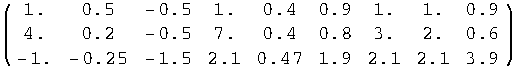
\includegraphics{refHmat.pdf}}}\intertext{with}
\psi_\epsilon=0, \,\,  \psi_z=I
\end{gather*}
(\footnote{{refHmat.pdf}})
These coefficients  happen to produce a unique stable solution.
\begin{gather*}
  B=
\vcenter{\hbox{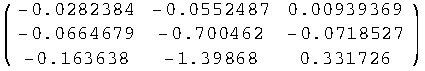
\includegraphics{refBmat.pdf}}}
\phi=
\vcenter{\hbox{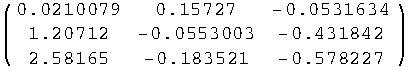
\includegraphics{refPhimat.pdf}}}\\
F=
\vcenter{\hbox{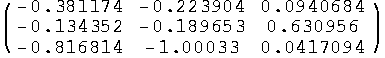
\includegraphics{refFmat.pdf}}}
\end{gather*} (\footnote{files generated by demoApprox.mth}\footnote{{refBmat.pdf}})(\footnote{{refPhimat.pdf}})(\footnote{{refFmat.pdf}})
We can use the family of conditional expectations
along with the contrived reference model to recover an 
approximation for equation \refeq{soln} along with error bounds.
\footnote{Note that the reference model is deterministic and the $z$ functions account for the stochastic nature of the model.}
% \footnote{
% We need not  make these adjustments for the steady state,
% but doing so economizes on the number of terms 
% required for a given level of approximation
% accuracy.}

Using the following parameter values

\begin{gather}
\vcenter{\hbox{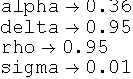
\includegraphics{RBCParamSubs.pdf}}} \,\, \text{ with } \,\,
  \begin{bmatrix}
    c_{ss}\\k_{ss} \\ \theta_{ss} \label{rbcparams}
  \end{bmatrix}=
\vcenter{\hbox{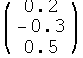
\includegraphics{RBCSSVal.pdf}}}
\end{gather}(\footnote{{RBCParamSubs.pdf}})(\footnote{{RBCSSVal.pdf}})

The contrived model can produce accurate values for the solution, but can require quite a few terms in the series to achieve a given level of accuracy. 
 Alternatively, as one might expect, developing 
a series using the model linearized about the ergodic mean produces a given
level of accuracy with 
fewer series terms.  

Note that the error bounds are useful in predicting how many terms are required for a given level of accuracy. Even the contrived model with randomly chosen
coefficients can achieve machine precision accuracy if one uses enough
terms from the series.  It also shows that adding new terms at some point becomes useless as rounding error limits any further improvement in the calculation.
This provides us some assurance that our iterative algorithm can be robust 
against errors if we include enough terms.

The table presents conservative estimates of the number of terms required
since the calculation uses the infinity norm.  I estimate the infinity
norm by using a global maximization method to compute the largest value
attained by the infinity norm of the equation errors.

We can develop a robust algorithm since we can compute how many terms
we must compute in order to guarantee a particular level of acuracy.
I computed the largest infinity norm for the product of h over a range of
reasonable values.  

Algorithm will allow us to construct approximation along with error bounds on the resulting approximations.\footnote{file generated by demoApprox.mth -- {truncErr.csv}}

\begin{table}
  \centering
\pgfplotstabletypeset[col sep=comma,
columns/0/.style={int detect,column name=N},
columns/1/.style={column name=Actual},
columns/2/.style={column name=Bound},
columns/3/.style={column name=Actual},
columns/4/.style={column name=Bound},
every head row/.style={before row={&\multicolumn{2}{c}{Arbitrary Model}&\multicolumn{2}{c}{Linearized RBC Model}\\}}
]{./truncErr.csv}

  \caption{Truncation Errors: Bound and Actual}
\label{truncTab}
\end{table}

  \subsection{The Problem Statement}

We will be interested in finding solutions for models that can be written in  the form


\begin{gather*}
  h_i(x_{t-1},x_{t},x_{t+1},\epsilon_t)=h^{det}_{io}(x_{t-1},x_{t},\epsilon_t)+\sum_{j=1}^{p_i} [h^{det}_{ij}(x_{t-1},x_{t},\epsilon_t)h^{nondet}_{ij}(x_{t+1})]=0
\end{gather*}
This is a very broad class of models and most economic models can 
be cast in this form.  

For example, the Euler equations for the  neoclassical growth  model 
\label{sec:simple-rbc-model-ext} can be written as
\begin{gather}
h_{10^{det}}(\cdot)=\frac{1}{c_t},\,\,
h_{11}^{det}()=\alpha \delta k_{t}^{\alpha-1} ,\,\,
h_{11}^{nondet}(\cdot)=E_t \left (\frac{\theta_{t+1}}{c_{t+1}} \right )\\
h_{20}^{det}(\cdot)=c_t + k_t-\theta_tk_{t-1}^\alpha,\,\,
h_{21}^{det}(\cdot)=0\\
h_{30}^{det}(\cdot)=\ln \theta_t -(\rho \ln \theta_{t-1} + \epsilon_t),\,\,
h_{31}^{det}(\cdot)=0
\end{gather}
Since we will be working with models where expectations are computed at time t, $\epsilon_t$ is known and the only stochastic components are those with time subscripts greater than $t$. We will need to compute 
the conditional expectation of nonlinear expressions,  
this specification will allow us to include auxiliary
variables that we will include in the augmented model for 
accurately recursively computing  the appropriate expected values.
Below, we will consider 
systems that augment these dynamic equations with additional constraints 
on the evolution of the variables.


We will be intersted in
finding a time invariant function $g^\ast$ that satisfies
\begin{gather}
  \begin{split}
h(x_{t+s-1},g^\ast(x_{t+s-1},\epsilon_{t+s}),\mathcal{H}[g^\ast(g^\ast(x_{t+s-1},\epsilon_{t+s}),\epsilon_{t+s+1})],\epsilon_{t+s}) \\
m(x_{t+s-1},g^\ast(x_{t+s-1},\epsilon_{t+s}),\mathcal{H}[g^\ast(g^\ast(x_{t+s-1},\epsilon_{t+s}),\epsilon_{t+s+1})],\epsilon_{t+s}) \ge 0  \label{theProblem}
  \end{split}
%  \intertext{define} 
% \mathcal{G}^\ast(x_{t+s-1},\epsilon_{t+s})= \mathcal{H}[g^\ast(g^\ast(x_{t+s-1},\epsilon_{t+s}),\epsilon_{t+s+1})] \nonumber
 \end{gather}
 for all $s>0$ where $\mathcal{H}$ is an operator, 
  that maps stochastic functions of $x$ and $\epsilon$ into deterministic 
functions of $x$ alone.  In this paper we will consider two such operators:


\begin{description}
\item[Perfect Foresight]
\begin{gather*}
     \mathcal{H}^{PF}[g^{k}(x,\epsilon_{t+T-k+1})]=
g^{k}(x,0)\\
\end{gather*}


\item[Rational Expectations] 
\begin{gather*}
     \mathcal{H}^{RE}[g^{k}(x,\epsilon_{t+T-k+1})]=
\mathcal{E}_t[g^{k}(x,\epsilon_{t+T-k+1})|x]\\
\end{gather*}

 \end{description}












In what follows, we will use a representation like equation \refeq{theTruncSeries} 
to construct a sequence of functions, $g^k$, 
that will approximate the typically unknown solution $g^\ast$.
If we knew $g^\ast$, and  these function generate a bounded family of 
trajectories, we could define $z(x_{t+s-1},\epsilon_t)$ using \refeq{defZ}.
Constructing a companion linear model would subsequently allow 
 us to write down a series representation for the $g^\ast$ functions.  Below, we will show how to ``reverse engineer'' the series representation for $g^\ast$.

\section{Constructing an Approximation}
\label{sec:constr-an-appr}

We begin by choosing some linear model of appropriate dimension that 
has a uniquely convergent steady state.  
Although this is not necessary, it may be possible to obtain this model by
linearizing the original model around the deterministic steady state.\footnote{As noted above, one could construct a series representation using any linear
 model of appropriate dimension with a unique stable solution.  The rate of convergence and the number of terms required for a  given level of accuracy will depend upon the linear model employed.}


 \begin{gather}
 g^0(x_{t-1},\epsilon_{t})=  
B x_{t-1}+ \phi \psi_\epsilon\epsilon_{t} +
 (I - F)^{-1} \phi \psi_c\\ \label{firstIter}
z^{0}_{t+i}(x_{t-1},\epsilon_{t-1})=0 \,\, \forall i \ge 0
 \end{gather}
We are now in a position to easily compute 
 \begin{gather}
\xIter{0}{x}=\mathcal{H}^{PF}[g^{0}(x,\epsilon_{t-k+1})]=
\mathcal{H}^{RE}[g^{0}(x,\epsilon_{t-k+1})]= 
B x+  (I - F)^{-1} \phi \psi_c
 \end{gather}
\begin{gather*}
\underbrace{x_{t-1},0} 
\underbrace{\xNow{0},\zNow{0}}
\underbrace{\xNowtp{0}=\xIter{0}{x_{t}},0}
\end{gather*}
In other words, from time t onwards, this approximation assumes 
that our stand-in
 convergent linear model completely characterizes the solution.\footnote{
The algorithm terminates with an approximation for 
the time invariant function $g^\ast$.}  It is unlikely that $g^0(x_{t-1},\epsilon_{t})$
satisfies equation \ref{theProblem} for arbitrary $x_{t-1}$ even for $s=0$.
We can get a pessimistic upper bound for how far we are away from the solution 
by computing the infinity norm of substituting the variables from into Equation \ref{theProblem}.\footnote{The values in Table \ref{truncTab} illustrate how
pessimistic this approximation can be, but it turns out we can expect the accuracy of  approximate truncation errors improve as we expand the approximation series.}

Next, we compute a solution in which the nonlinear equations are satisfied at time t alone while the stand-in linear system holds sway subsequently.
Our algorithm will  compute
\begin{gather*}
\underbrace{x_{t-1},0} 
\underbrace{\xNow{1},\zNow{1}}
\underbrace{\xNowtp{1}=\xIter{1}{x_{t+1}},0}
\underbrace{\xNowtp{1}=\xIter{0}{x_{t+1}},0}
\end{gather*}
that satisfy the nonlinear equation system at time t.
For a given $x_{t-1}$, we substitute
\begin{gather}
x_{t-1}, \,\,
  x_t=B x_{t-1} + \phi z^1(x_{t-1},\epsilon_t) , \,\,
  x_{t+1}=B x_{t} + \phi \mathcal{Z}^1(x_t)
\end{gather}
into the non linear equation system to determine the 
$z^1(x_{t-1},\epsilon_t)$ and consequently $x_t^1(x_{t-1},\epsilon_t)$.
We then have
 \begin{gather}
 g^1(x_{t-1},\epsilon_{t})=  
B x_{t-1}+ \phi \psi_\epsilon\epsilon_{t} +
\phi \psi_\epsilon z^1(x_{t-1},\epsilon_t)+
 (I - F)^{-1} \phi \psi_c\\ \label{firstIter}
z^{1}_{t+i}(x_{t-1},\epsilon_{t-1})=0 \,\, \forall i \ge 1
 \end{gather}
Now, $g^1(x_{t-1},\epsilon_{t})$
satisfies equation \ref{theProblem} for arbitrary $x_{t-1}$ at time $t$ with $s=0$.  However, it probably does not solve the system for $s>0$.
We can get a pessimistic upper bound for how far we are away from the solution 
by substituting the variables and computing the infinity norm for plausible values of $x_{t-1}$.
\begin{gather}
\xNow{1},\xNowtp{1},\xNowtp{1}=\xIter{1}{x_{t+1}}
\end{gather}
into Equation \ref{theProblem}. If the accuracy of the approximation is adequate, we need not compute any further  terms in the power series.  If not,
we are now in a position to compute our choice of
$\mathcal{Z}^1(x)=\mathcal{H}^{PF}[g^{1}(x,\epsilon_{t-k+1})]$ or
$\mathcal{Z}^1(x)=\mathcal{H}^{RE}[g^{1}(x,\epsilon_{t-k+1})]$.

%  \begin{gather}
%  g^0(x_{t-1},\epsilon_{t})=  
% B x_{t-1}+ \phi \psi_\epsilon\epsilon_{t} +
%  (I - F)^{-1} \phi \psi_c\\ \label{firstIter}
% z^{0}_{t+i}(x_{t-1},\epsilon_{t-1})=0 \,\, \forall i \ge 0
%  \end{gather}
%  \begin{gather}
%  g^0(x_{t-1},\epsilon_{t})=  
% B x_{t-1}+ \phi \psi_\epsilon\epsilon_{t} +
%  (I - F)^{-1} \phi \psi_c\\ \label{firstIter}
% z^{0}_{t+i}(x_{t-1},\epsilon_{t-1})=0 \,\, \forall i \ge 0
%  \end{gather}

Using these functions we can then compute a solution for a model whose trajectories satisfy equation system \refeq{rbcSys}
for two time periods and satisfy equation \refeq{rbcLinSys} subsequently.

\begin{gather}
\underbrace{x_{t-1},0}
\underbrace{\xNow{2},\zNow{2}} 
\underbrace{\xNowtp{2}=\XNow{2}{t}{t},\ZNow{2}{1}{t}}
\underbrace{\XNow{1}{t+1}{t},0}\underbrace{\XNow{0}{t+2}{t+1},0}    \intertext{where we have solved for $\xNow{2}$ and $\zNow{2}$ to satisfy the  equation system \ref{theProblem}.}
\xNowtp{2}=\XNow{1}{t}{t}
\end{gather}

\begin{gather}
  \label{eq:1}
  x_t=B x_{t-1} + \phi z^2(x_{t-1},\epsilon) + F \phi \mathcal{Z}^1(x_t)\\
  x_{t+1}=B x_{t} + \phi \mathcal{Z}^1(x_t)+
 (I - F)^{-1} \phi \psi_c\\
  x_{t+2}=B x_{t+1} + (I - F)^{-1} \phi \psi_c\\
  x_{t+3}=B x_{t+2} + (I - F)^{-1} \phi \psi_c
\end{gather}

The next iteration highlights an aspect of the algorithmic step which allows us
to continue to exploit the law of iterated expectations in discoving the
solution for the model.
{\small
\begin{gather}
\underbrace{x_{t-1},0}
\underbrace{\xNow{3},\zNow{3}} 
\underbrace{\xNowtp{3}=\XNow{3}{t}{t},\ZNow{3}{1}{t}} 
\underbrace{\XNow{2}{t+1}{t},\ZNow{2}{2}{t+1}} 
\underbrace{\XNow{1}{t+3}{t+2},0}
\underbrace{\XNow{0}{t+4}{t+3},0}
\end{gather}
}

\begin{gather}
  \label{eq:1}
  x_t=B x_{t-1} + \phi z^3(x_{t-1},\epsilon) + F \phi \mathcal{Z}^2(x_t)+ F^2 \phi \mathcal{Z}^1(x_t)+
 (I - F)^{-1} \phi \psi_c\\
  x_{t+1}=B x_{t} + \phi \mathcal{Z}^1(x_t)+ F^2 \phi \mathcal{Z}^1(x_t)+
 (I - F)^{-1} \phi \psi_c\\
  x_{t+2}=B x_{t+1} + (I - F)^{-1} \phi \psi_c\\
  x_{t+3}=B x_{t+2} + (I - F)^{-1} \phi \psi_c\\
  x_{t+4}=B x_{t+2} + (I - F)^{-1} \phi \psi_c
\end{gather}



In the general iteration step we will have
\begin{gather}
  \label{eq:1}
  x_t=B x_{t-1}  \phi \psi_\epsilon \epsilon_t + (I - F)^{-1} \phi \psi_c +
\sum_{s=0}^{k} F^s \phi \mathcal{Z}^{k-s}(x_{t+s}^{k+1})\\
  x_{t+s}^{k+1}=\Pi_{s=0}^k \xIter{s}{ x_{t}^{k+1}}
\end{gather}


\section{Restatement}

Define $\XZPair{0}\equiv(B x_{t-1}+ \phi \psi_\epsilon\epsilon_{t} +
 (I - F)^{-1} \phi \psi_c,0)$.

Now, given
\begin{gather}
  \{\XZPair{0},\ldots,\XZPair{k}\}\intertext{ find }
\zNow{k+1} \ni \xNow{k+1} \intertext{satisfies Equation \ref{theProblem} where}
  \xNow{k+1}\equiv B x_{t-1} + \phi \psi_\epsilon \epsilon_t + (I - F)^{-1} \phi \psi_c +  \phi \zNow{k+1}+
  \begin{cases}
0& \mbox{if }k=0\\    
\sum_{s=1}^{k} F^s \phi  \mathcal{Z}^{k-s}(x_{t+s}^k)&\mbox{if } k>0
  \end{cases}
\\
  x_{t+s}^{k+1}=\xIter{p}{ x_{t+s-1}^{k+1}}
  \begin{cases}
p=k+1-s &1\le s\le k+1\\
p=0 &s> k+1
  \end{cases}\intertext{to construct}
\ZNow{k+1}{}{}\equiv\mathcal{H}^{PF}[\zNow{k+1}] \text{ and }
\XNow{k+1}{}{}\equiv\mathcal{H}^{PF}[\xNow{k+1}] 
\intertext{ or }
\ZNow{k+1}{}{}\equiv\mathcal{H}^{RE}[\zNow{k+1}]\text{ and }
\XNow{k+1}{}{}\equiv\mathcal{H}^{RE}[\xNow{k+1}]
\end{gather}

\section{Examples}
\label{sec:examples}

\anEdit{models should be well known.  Avoid spending time explaining a model.
Luca's JME paper 3rd model.\cite{Guerrieri2015}}

\anEdit{Explore what others have said about error bounds.  }

\subsection{A Simple RBC Model}
\label{sec:simple-rbc-model-1}

We construct our stand-in model by augmenting the model with the equation
\begin{gather*}
  \rcpC_t=\frac{1}{c_t}
\end{gather*}
substituting $\rcpC_{t+1}$ for $\frac{1}{c_{t+1}}$ in the first equation and 
 linearizing the RBC model about the ergodic mean
given in \refeq{rbcparams}
\begin{gather}
  \begin{bmatrix}
H_{-1}&H_{0}&H_{1} 
  \end{bmatrix}=
\vcenter{\hbox{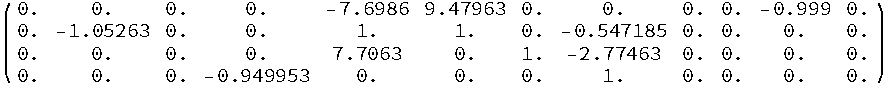
\includegraphics{RBCHmatSymb.pdf}}} \label{rbcLinSys}
\intertext{with}
\psi_\epsilon=
\begin{bmatrix}
  0\\0\\1\\0
\end{bmatrix}, \psi_z=I
\end{gather}(\footnote{generated by AMAPaperCalcs.mth {RBCHmatSymb.pdf}})

These coefficients  produce a unique stable linear solution.

\begin{gather*}
  B=
\vcenter{\hbox{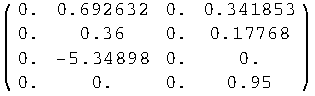
\includegraphics{RBCBmatSymb.pdf}}},
\phi=
\vcenter{\hbox{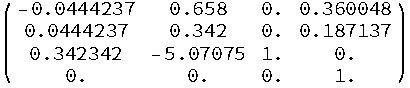
\includegraphics{RBCPhimatSymb.pdf}}}\\
F=
\vcenter{\hbox{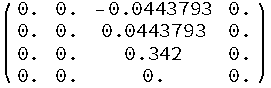
\includegraphics{RBCFmatSymb.pdf}}}\\
\psi_c=
\vcenter{\hbox{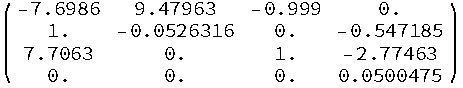
\includegraphics{RBCHSum.pdf}}}
\vcenter{\hbox{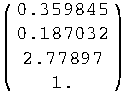
\includegraphics{RBCSS.pdf}}}=\vcenter{\hbox{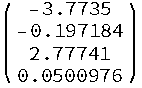
\includegraphics{RBCPsissSymb.pdf}}}
\end{gather*}(\footnote{generated by AMAPaperCalcs.mth {RBCBmatSymb.pdf}})(\footnote{generated by AMAPaperCalcs.mth {RBCPhimatSymb.pdf}})(\footnote{generated by AMAPaperCalcs.mth {RBCFmatSymb.pdf}})(\footnote{generated by AMAPaperCalcs.mth {RBCHSum.pdf}})(\footnote{generated by AMAPaperCalcs.mth {RBCSS.pdf}})

Applying the formula \refeq{firstIter} produces:

{\tiny
\begin{gather*}
  \begin{bmatrix}
c_t\\k_t\\ \rcpC_t\\\theta_t
  \end{bmatrix}=%paperCalcsRBCExample xt00
   \left(
   \begin{array}{c}
 0.359845 \epsilon _t+0.692632 k_{t-1}+0.341853 \theta _{t-1}-0.0442851
   \text{z1}_{t-1}+0.658 \text{z2}_{t-1}+0.359845 \text{z3}_{t-1}-0.111552 \\
 0.187032 \epsilon _t+0.36 k_{t-1}+0.17768 \theta _{t-1}+0.0442851
   \text{z1}_{t-1}+0.342 \text{z2}_{t-1}+0.187032 \text{z3}_{t-1}-0.0579799 \\
 -5.34898 k_{t-1}+0.342 \text{z1}_{t-1}-5.08153
   \text{z2}_{t-1}+\text{z4}_{t-1}+3.7794 \\
 \epsilon _t+0.95 \theta _{t-1}+\text{z3}_{t-1}+0.05 \\
   \end{array}
   \right)
\end{gather*}
}

and 


{\tiny
%xt01=Private`computeNextXt[{Private`bmat,Private`phimat,Private`fmat,Private`psieps,Private`psic,Private`psiz},solnFunc00PF[[3+Range[3]]],{{cc},{kk},{tt}},{1}]//N//Expand//Simplify
\begin{gather*}
  \begin{bmatrix}
c_{t+1}\\k_{t+1}\\ \rcpC_{t+1}\\\theta_{t+1}
  \end{bmatrix}=%paperCalcsRBCExample xt00
  \left(
   \begin{array}{c}
 0.471397 \epsilon _t+0.249347 k_{t-1}+0.447827 \theta _{t-1}+0.0306732
   \text{z1}_{t-1}+0.23688 \text{z2}_{t-1}+0.471397 \text{z3}_{t-1}-0.134618 \\
 0.245012 \epsilon _t+0.1296 k_{t-1}+0.232761 \theta _{t-1}+0.0159426
   \text{z1}_{t-1}+0.12312 \text{z2}_{t-1}+0.245012 \text{z3}_{t-1}-0.0699687 \\
 -1.00043 \epsilon _t-1.92563 k_{t-1}-0.950409 \theta _{t-1}-0.23688
   \text{z1}_{t-1}-1.82935 \text{z2}_{t-1}-1.00043 \text{z3}_{t-1}+4.08954 \\
 0.95 \epsilon _t+0.9025 \theta _{t-1}+0.95 \text{z3}_{t-1}+0.0975 \\
   \end{array}
   \right)
\end{gather*}}

Substituting  these expressions into equation \refeq{rbcSys} produces
a deterministic system such that, given specific values for 
$(x_{t-1},\epsilon_{t})=(c_{t-1}, k_{t-1},\rcpC_{t-1}, \theta_{t-1}, \epsilon_t)$, we can solve for $z_{1t}(x_{t-1},\epsilon_{t})$, $z_{2t}(x_{t-1},\epsilon_{t})$, $z_{2t}(x_{t-1},\epsilon_{t})$, and $z_{4t}(x_{t-1},\epsilon_{t})$  completely determining
$c_{t}(x_{t-1},\epsilon_{t})$, $k_{t}(x_{t-1},\epsilon_{t})$, $\rcpC_{t}(x_{t-1},\epsilon_{t})$  and $\theta_{t}(x_{t-1},\epsilon_{t})$.\footnote{In this example, the lagged value,  $c_{t-1}$ does not appear in the equation system and consequently plays no role in determining the solution.}  In effect we have 
computed a solution for a model whose trajectories satisfy equation system \refeq{rbcSys}
for one time period and satisfy equation \refeq{rbcLinSys} subsequently. As can
be seen in the top panel of Figure \ref{fig:cfuncfirst}, 
imposing the constraint for even a single period captures much of the nonlinearity, but the bottom panel shows that the solution is 
still significantly far away from the exact solution.

\begin{figure}
  \centering
%\includegraphics{cFuncExt00Lin.pdf}(\footnote{{cFunc00Lin.pdf}})
  \caption{Solution for c imposing non linear model constraints for a single period}
%\includegraphics{cFuncExt00Exact.pdf}(\footnote{{cFunc00Exact.pdf}})
  \caption{Solution for c imposing non linear model constraints for a single period}
  \label{fig:cfuncfirst}
\end{figure}

We are now in a position to compute
$\mathcal{H}^{PF}[g^{0}(x,\epsilon_{t-k+1})]$ or
$\mathcal{H}^{RE}[g^{0}(x,\epsilon_{t-k+1})]$.
Using these functions we can then compute a solution for a model whose trajectories satisfy equation system \refeq{rbcSys}
for two time periods and satisfy equation \refeq{rbcLinSys} subsequently.
\begin{gather}
  \label{eq:1}
  x_t=B x_{t-1} + \phi z_0(x_{t-1},\epsilon) + F \phi \mathcal{Z}^1(x_t)\\
  x_{t+1}=B x_{t} + \phi \mathcal{Z}^1(x_t)
\end{gather}
{\tiny

\begin{gather}%paperCalcsRBCExample.mth xt01
  \label{eq:2}
   \left(
   \begin{array}{c}
 0.359845 \epsilon _t+0.692632 k_{t-1}+0.341853 \theta _{t-1}-0.0442851
   \text{z1}_{t-1}-0.0442851 \text{Z1}_{t-1}+0.658 \text{z2}_{t-1}+0.359845
   \text{z3}_{t-1}+0.225036 \text{Z3}_{t-1}-0.0151455 \text{Z4}_{t-1}-0.111552 \\
 0.187032 \epsilon _t+0.36 k_{t-1}+0.17768 \theta _{t-1}+0.0442851
   \text{z1}_{t-1}+0.0442851 \text{Z1}_{t-1}+0.342 \text{z2}_{t-1}+0.187032
   \text{z3}_{t-1}-0.225036 \text{Z3}_{t-1}+0.0151455 \text{Z4}_{t-1}-0.0579799 \\
 -5.34898 k_{t-1}+0.342 \text{z1}_{t-1}+0.342 \text{Z1}_{t-1}-5.08153
   \text{z2}_{t-1}-1.73788 \text{Z3}_{t-1}+\text{z4}_{t-1}+0.116964
   \text{Z4}_{t-1}+3.7794 \\
 \epsilon _t+0.95 \theta _{t-1}+\text{z3}_{t-1}+0.05 \\
   \end{array}
   \right)
\end{gather}
}

{\tiny
  \begin{gather}
    \label{eq:3}
       \left(
   \begin{array}{c}
 0.471397 \epsilon _t+0.249347 k_{t-1}+0.447827 \theta _{t-1}+0.0306732
   \text{z1}_{t-1}-0.0578969 \text{Z1}_{t-1}+0.23688 \text{z2}_{t-1}+0.658
   \text{Z2}_{t-1}+0.471397 \text{z3}_{t-1}+0.429014 \text{Z3}_{t-1}-0.00465525
   \text{Z4}_{t-1}-0.134618 \\
 0.245012 \epsilon _t+0.1296 k_{t-1}+0.232761 \theta _{t-1}+0.0159426
   \text{z1}_{t-1}+0.104513 \text{Z1}_{t-1}+0.12312 \text{z2}_{t-1}+0.342
   \text{Z2}_{t-1}+0.245012 \text{z3}_{t-1}-0.119017 \text{Z3}_{t-1}+0.0205979
   \text{Z4}_{t-1}-0.0699687 \\
 -1.00043 \epsilon _t-1.92563 k_{t-1}-0.950409 \theta _{t-1}-0.23688
   \text{z1}_{t-1}+0.44712 \text{Z1}_{t-1}-1.82935 \text{z2}_{t-1}-5.08153
   \text{Z2}_{t-1}-1.00043 \text{z3}_{t-1}-0.534171 \text{Z3}_{t-1}+1.03595
   \text{Z4}_{t-1}+4.08954 \\
 0.95 \epsilon _t+0.9025 \theta _{t-1}+0.95 \text{z3}_{t-1}+\text{Z3}_{t-1}+0.0975 \\
   \end{array}
   \right)
  \end{gather}
}

\begin{figure}
  \centering
%\includegraphics{cFuncTwoPerErr.pdf}(\footnote{{cFuncTwoPerErr.pdf}})
  \caption{Solution for c imposing non linear model constraints for two periods}
%\includegraphics{cFuncThreePerErr.pdf}(\footnote{{cFuncThreePerErr.pdf}})
  \caption{Solution for c imposing non linear model constraints for three periods}
  \label{fig:cfuncsecond}
\end{figure}




% \begin{figure}
%   \centering
%\includegraphics{cFunc00PF.pdf}(\footnote{{cFunc00PF.pdf}})
%   \caption{Perfect foresight solution for c imposing non linear model constraints for a single period}
%   \label{fig:cfuncfirstpf}
% \end{figure}

% \begin{gather}
%   \label{eq:1}
%   x_t=B x_{t-1} + \phi z_0(x_{t-1},\epsilon) + F \phi \mathcal{Z}^1(x_t)+  F^2 \phi \mathcal{Z}^2(x_t)\\
%   x_{t+1}=B x_{t} + \phi \mathcal{Z}^1(x_t) + F \phi \mathcal{Z}^2(x_t)
% \end{gather}




\subsection{A Simple Financial Model}
\label{sec:simple-financ-model}

A model specification consists of
\begin{description}
\item[Uniquely convergent linear rational expectations model] 
We will need the $B, \phi, F, \psi_\epsilon, \psi_c \text{ and }\psi_z$ matrices
\item[A function that computes the current set of constraint given a path and the current set of z functions] 
  \begin{gather*}
    \mathcal{C}(x_{t-1},x_{t},x_{t+1},z(x_{t-1},\epsilon_t))
  \end{gather*}
\end{description}
\subsection{A Regime Switching Model}
\label{sec:regime-switch-model}



\cite{foerster13}

\begin{gather*}
c_t + z_t k_t = z_t^{1-\alpha} k_{t-1}^\alpha + (1-\delta)k_{t-1}\\
 \log z_t = (1-\rho(s_t))\mu(s_t) + \rho(s_t)\log z_{t-1}+ \sigma(s_t) \epsilon_t\\
 c_t^{\gamma-1} = \beta  
 E_t ( c_{t+1}^{\gamma-1} (\alpha z_{t+1}^{1-\alpha} k_t^{\alpha -1} + (1-\delta) ))
\end{gather*}



\section{Implementation Details }
\label{sec:implementation}



\begin{itemize}
\item there could be alternative solutions along the way to computing the path that lead to dead ends and frustrate convergence -- even if only one unique time invariant solution.
\item which is better to characterize discrepancy, simulation via decision rule or discrepancy between the ``computed exact'' solution path  do they coalesce
\item parallelization
\item improve simulation performance via z feedback
\item One need only construct and solve a system large enough to determine the non zero $z$-function.
\item any linear equation required to remains satisfied will have an identically zero z
\item for non linear variables that are completely backward looking one can solve for the z functions for those equations 
ahead of time( as well as just substitute them out )
\item use function composition evaluation to determine refined grid. possible that the set of refinements produce a fixed point  ( probably gives especially accurate interpolation
\item lots of choices about choosing grid pointseach z could have different interpolation order or even mix chebyshev and interpolation
\item Law of iterated expectations
\item Interpolate before or after integration

  \begin{gather}
    E_t(X) = E_t(E_{t+1}(X))
  \end{gather}
\end{itemize}
  






\appendix
\newpage

     
\section{The algorithms}
\label{sec:algorithms}

\begin{pseudocode}{solnSubs}{[c_{t-1},k_{t-1},\frac{1}{c_t},\theta_{t-1},\epsilon_t]}
\RETURN{Rules}  
\end{pseudocode}


\begin{pseudocode}{solnFuncs}{[\{c_{t-1},k_{t-1},\frac{1}{c_t},\theta_{t-1},\epsilon_t\}]}
\RETURN{Matrix}  
\end{pseudocode}

 \begin{gather}
 Through[funcsInterp[k_{t-1},\theta_{t-1},\epsilon_t] \rightarrow
 \begin{bmatrix}
   x_t\\x_{t+1}\\z_t
 \end{bmatrix}
 \\
 Through[funcsInterpPF[k_{t-1},\theta_{t-1}]\rightarrow
 \begin{bmatrix}
   x_t\\x_{t+1}\\z_t
 \end{bmatrix}
\\
 Through[funcsInterpRE[k_{t-1},\theta_{t-1}]\rightarrow
 \begin{bmatrix}
   x_t\\x_{t+1}\\z_t
 \end{bmatrix}
\\
 Through[ZZks[k_{t-1},\theta_{t-1}]\rightarrow
 \begin{bmatrix}
z_t
 \end{bmatrix}
\\
 \end{gather}


% \section{Things To Do}
% \label{sec:things-do}

% \begin{itemize}
% \item guess should also use shock
% \item code to check model definition functions' validity
% \item flesh out constraints on function in code and add to text
% \item describe fixed point and init guess  need to take account of shock to get fixedpoint to converge
%\item Volterra Series and Impulse Response Functions
% \end{itemize}

\section{Truncation Error Bounds}
\label{truncForm}
{
\begin{gather*}
\phi \psi_c=  \sum_{s=0}^\infty F^s \phi \psi_c  -   F \sum_{s=0}^\infty F^s \phi \psi_c \\
(I-F) \left (\sum_{s=0}^\infty F^s \phi \psi_c \right ) =\phi \psi_c\\
\sum_{s=0}^\infty F^s \phi \psi_c=(I - F)^{-1}\phi \psi_c\\
\sum_{s=0}^{k+1} F^s \phi \psi_c=F \sum_{s=0}^{k} F^s \phi \psi_c + \phi \psi_c\\
F^{k+1} \phi \psi_c +\sum_{s=0}^{k} F^s \phi \psi_c=F \sum_{s=0}^{k} F^s \phi \psi_c + \phi \psi_c\\
(I -F)\sum_{s=0}^{k} F^s\phi \psi_c  = (I- F^{k+1}) \phi \psi_c\\
\sum_{s=0}^{k} F^s \phi \psi_c = (I -F)^{-1}(I- F^{k+1}) \phi \psi_c\\
\sum_{s=k+1}^{\infty} F^s \phi \psi_c = (I -F)^{-1} F^{k+1}\phi \psi_c
\end{gather*}
}

\section{Probably Not Needed}


 \begin{gather}
 g^0(x_{t+T-1},\epsilon_{t+T})=  
B x_{t+T-1}+ \phi \psi_\epsilon\epsilon_{t+T} +
 (I - F)^{-1} \phi \psi_c\\ \label{firstIter}
z^{T,0}_{t+T+i}(x_{t+T-1},\epsilon_{t+T-1})=0 \,\, \forall i \ge 0
 \end{gather}
In other words, this approximation assumes 
that our stand-in convergent linear model completely characterizes the solution.\footnote{
The algorithm terminates with an approximation for 
the time invariant function $g^\ast$. }

 Our algorithm will use  
 \begin{gather*}
 g^{k}(x_{t+T-(k+1)},\epsilon_{t+T-k}) \intertext{ and}
 \{ z^{T-k,k}(x_{t+T-(k+1)},\epsilon_{t+T-k}),\ldots, z^{T,k}(x_{t+T-(k+1)},\epsilon_{t+T-k})\}
   \end{gather*}
  to solve for 
 \begin{gather*}
 g^{k+1}(x_{t+T-(k+2)},\epsilon_{t+T-(k+1)}) \intertext{ and}
 \{ z^{T-(k+1),k+1}(x_{t+T-(k+2)},\epsilon_{t+T-(k+1)}),\ldots, z^{T,k+1}(x_{t+T-(k+2)},\epsilon_{t+T-(k+1)})\}
   \end{gather*}





First, note that after completing any given step $k$
we  are in a position to compute the deterministic functions 
$\mathcal{G}^k$ and $\{\mathcal{Z}^{T-k,k},\ldots,\mathcal{Z}^{T,k}\}$:
\begin{gather*}
   \mathcal{G}^{k}(x)= \mathcal{H}[g^{k}(x,\epsilon_{t+T-k+1})]\\
   \mathcal{Z}^{T-k+i,k}(x)= \mathcal{H}[z^{T-k+i,k}(x,\epsilon_{t+T-k+1})] \,\, i=0,\ldots,k. 
\end{gather*} 

The iteration step proceeds as follows:

\begin{enumerate}
\item Write
\begin{align*}
g^{k+1}(x_{t+T-(k+2)},\epsilon_{t+T-(k+1)})=&\\
&B x_{t-1}+ \phi \psi_\epsilon\epsilon_t + \\
&\sum_{s=0}^{k+1} F^s \phi z^{T-(k+1)+s,k+1}_{t+s}(x_{t+T-(k+2)},\epsilon_{t+T-(k+1)}) +\\
& (I - F)^{-1} \phi \psi_c
\end{align*}
\item economize on updating some of
the $z^{T-k+i,k+1}(x_{t+T-(k+2)},\epsilon_{t+T-(k+1)})$ by composing known
deterministic functions with the as yet undetermined $g^{k+1}$
\begin{gather*}
z^{T-k+i,k+1}(x_{t+T-(k+2)},\epsilon_{t+T-(k+1)})= \mathcal{Z}^{T-k+i,k}(g^{k+1}(x_{t+T-(k+2)},\epsilon_{t+T-(k+1)}) \,\, \\i=0,\ldots,k  
\end{gather*}
 and
\item  use the functions in \refeq{theProblem} to determine the new functions 
 $g^{k+1}$  and  $z^{T-(k+1),k+1}$ %(x_{t+T-(k+2)},\epsilon_{t+T-(k+1)})


\begin{gather*}
 h(x_{t+T-(k+2)},g^{k+1}(x_{t+T-(k+2)},\epsilon_{t+T-(k+1)}), \mathcal{G}^{k}(g^{k+1}(x_{t+T-(k+2)},\epsilon_{t+T-(k+1)})),\epsilon_{t+T-(k+1)})\\
m(x_{t+T-(k+2)},g^{k+1}(x_{t+T-(k+2)},\epsilon_{t+T-(k+1)}),\mathcal{G}^{k}(g^{k+1}(x_{t+T-(k+2)},\epsilon_{t+T-(k+1)})),\epsilon_{t+T-(k+1)}) \ge 0\\ \label{iterSys}
 g^{k+1}(x_{t+T-(k+2)},\epsilon_{t+T-(k+1)})= 
 B x_{t+T-(k+2)}+ \phi \psi_\epsilon\epsilon_{t+T-(k+1)} +\\
\sum_{i=1}^k F^i \phi \mathcal{Z}^{T-k+i,k}(g^{k+1}(x_{t+T-(k+2)},\epsilon_{t+T-(k+1)})) +\\
 \phi z^{(T-(k+1)),k+1}_{t+i+(k+1)}(x_{t+T-(k+2)},\epsilon_{t+T-(k+1)})\\
   \end{gather*}
\end{enumerate}

These steps will likely take place point by point and will require an interpolation or projection method to characterize the functions.

To determine $g_0(x_{t-1},\epsilon_t)$ we set

\begin{gather*}
	 g_{0}(x_{t-1},\epsilon_t) =B x_{t-1}+ \phi \psi_\epsilon\epsilon_t + (I - F)^{-1} \phi \psi_c + \phi z^{T,0}_{T}(x_{t-1},\epsilon_t)
\\
	 \mathcal{G}^0(x) =B x + (I - F)^{-1} \phi \psi_c \nonumber
\end{gather*}

and use  equation \refeq{iterSys} to determine the unknown $z_T(x_{T-1},\epsilon_T)$

\begin{gather*}
 h(x_{t+T-1},\mathbf{x}_T,\mathbf{x}_{T+1},\epsilon_{t+T})=0\\
 m(x_{t+T-1},\mathbf{x}_T,\mathbf{x}_{T+1},\epsilon_{t+T}) \ge 0\\
 \intertext{ where }
\mathbf{x}_t=B x_{T-1}+ \phi \psi_\epsilon\epsilon_t + (I - F)^{-1} \phi \psi_c+ \phi z^{T,0}_{T}(x_{T-1},\epsilon_t)\\
\mathbf{x}_{t+1}=B(B x_{T-1}+ \phi \psi_\epsilon\epsilon_t + (I - F)^{-1} \phi \psi_c + \phi z^{T,0}_{T}(x_{T-1},\epsilon_t)) + (I - F)^{-1} \phi \psi_c\\
   \end{gather*}




\begin{gather*}
  \{g_k(x_{t-1},\epsilon_t),\mathcal{Z}^k_0(x), \ldots, \mathcal{Z}^{k-1}_k(x) \} \rightarrow \\
  \{g^{k+1}(x_{t-1},\epsilon_t),\mathcal{Z}^{k+1}_0(x), \ldots, \mathcal{Z}^{k}_{k+1}(x) \}
\end{gather*}

The code employs a simple fixed point iteration for any given $x_{t-1},\epsilon_t$.
We begin by setting $[\prescript{0}{}{x}(x_{t-1},\epsilon_t)]=g_k(x_{t-1},\epsilon_t)$. We 
solve for $[\prescript{l+1}{}{x}(x_{t-1},\epsilon_t)]$ and $[\prescript{l+1}{}{z}(x_{t-1},\epsilon_{t})]$ in 


\begin{gather*}
\{ h, m, B, \phi, F, \psi_\epsilon, \psi_z \}  \rightarrow\\
 h(x_{t-1},[\prescript{l+1}{}{x}(x_{t-1},\epsilon_{t})], \mathcal{G}^{k}([\prescript{l}{}{x}(x_{t-1},\epsilon_{t})]),\epsilon_{t})\\
m(x_{t-1},[\prescript{l+1}{}{x}(x_{t-1},\epsilon_{t})],\mathcal{G}^{k}([\prescript{l}{}{x}(x_{t-1},\epsilon_{t})]),\epsilon_{t}) \ge 0\\
 [\prescript{l+1}{}{x}(x_{t-1},\epsilon_{t})]= 
 B x_{t-1}+ \phi \psi_\epsilon\epsilon_{t} +\\
\sum_{i=1}^k F^i \phi \mathcal{Z}^{k}_i(\mathbf{x}) +\\
 \phi [\prescript{l+1}{}{z}(x_{t-1},\epsilon_{t})]\intertext{ where}
\mathbf{x}=[\prescript{l+1}{}{x}(x_{t-1},\epsilon_{t})]\text{ or } [\prescript{l}{}{x}(x_{t-1},\epsilon_{t})]
   \end{gather*}


We terminate when 
\begin{gather*}
    \twoNorm{  \begin{bmatrix}
\prescript{l+1}{}{x}(x_{t-1},\epsilon_{t})-
\prescript{l}{}{x}(x_{t-1},\epsilon_{t})\\
\prescript{l+1}{}{z}(x_{t-1},\epsilon_{t})-
\prescript{l}{}{z}(x_{t-1},\epsilon_{t})
  \end{bmatrix}} \le \epsilon_{fp} = 10^{-10} \intertext{ with }
\begin{bmatrix}
{\hat{x}}(x_{t-1},\epsilon_{t})\\
{\hat{z}}(x_{t-1},\epsilon_{t})
\end{bmatrix}=
\begin{bmatrix}
\prescript{l+1}{}{x}(x_{t-1},\epsilon_{t})\\
\prescript{l+1}{}{z}(x_{t-1},\epsilon_{t})
\end{bmatrix}
\end{gather*}

We compute 
$  \hat{g}(x_{t-1},\epsilon_{t})$ by either projection or interpolation.



\newpage

\href{http://www.dynare.org/DynareShanghai2013/deterministic.pdf}{Occasionally binding constraints in neoclassical growth model}

 \bibliographystyle{plainnat}
 \bibliography{../../bibFiles/anderson,../../bibFiles/files}

\end{document}


